\section{Exercise four}

Consider the provided datasets:
\begin{figure}[H]
    \centering
    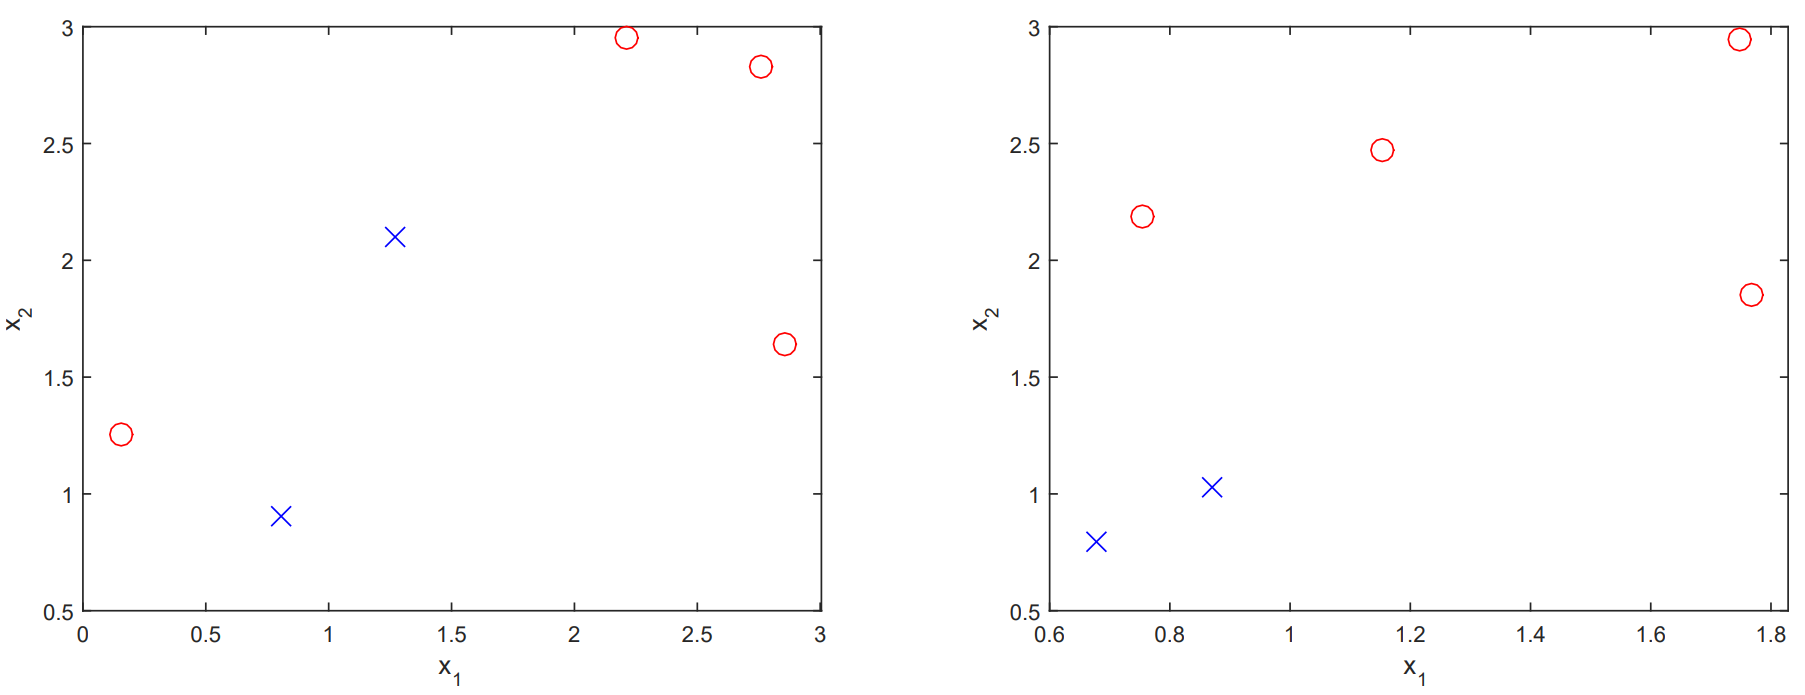
\includegraphics[width=0.75\linewidth]{images/class.png}
\end{figure}
Now, let's analyze whether the learning procedure terminates and the number of steps required for convergence using the online stochastic gradient descent algorithm to train a perceptron.

\subsection*{Solution}
The perceptron learning algorithm converges if there exists a linear separation hyperplane. In such a scenario, the classification error can be reduced to zero. 
If no linear separation exists, the optimization process doesn't halt. 
The convergence rate isn't assured since it relies on the initial parameterization and the sequence of points used for training. 
Nonetheless, convergence does occur within a finite number of steps.

In the first dataset (left), convergence isn't guaranteed. 
However, in the second dataset (right), the online stochastic gradient descent will ultimately converge within a finite number of steps.

Considering that the loss function for logistic regression is convex, the online learning process converges to the global optimum asymptotically, irrespective of the dataset provided.